\chapter{Preliminaries}
\label{chap:ch2}
In order to design intervention for human users, first we need to model human user behavior in some environment. 
We use the automated planning formalism \cite{nau2004} to describe the tasks the user performs in both the cyber-security and Rush Hour domains. 
The automated planning formalism is based on concepts such as goals, states and actions, to describe the behavior of rational agents. 
Although human user behavior is more complex than that of a rational agent, in our intervention models we assume the actor being intervened is a (bounded) rational agent.
In this chapter, we first present an overview of automated planning and describe how a state/action model can be represented as a classical planning problem. Next, we discuss the problem of inferring the intention of an agent and discuss three variants of the problem: plan recognition, goal recognition and activity recognition. Finally, we present a discussion on the existing literature on intention recognition considering a three-dimensional framework: number of agents in the environment, online/offline recognition and how the recognizer interacts with the environment during the intention recognition process.

\section{Automated Planning}
Planning aims at achieving some predefined objectives through a deliberation process that chooses and organizes actions by anticipating their outcomes. The planning formalism views the problem as a state transition system, defined as a tuple $\Sigma=(S,A,E,\gamma)$ where:
\begin{itemize}
\item $S = \lbrace s_1, s_2, \ldots \rbrace$ is a finite or recursively enumerable set of states;
\item $A = \lbrace a_1, a_2, \ldots \rbrace$ is a finite or recursively enumerable set of actions;
\item $E = \lbrace e_1, e_2, \ldots \rbrace$ is a finite or recursively enumerable set of events; and
\item $\gamma: S\times(A\cup E)\mapsto 2^S$ is a state transition function.
\end{itemize}
Given an action $a\in A$ and $\gamma(s,a)\neq\emptyset$, then $a$ is \textit{applicable} in state $s$. If $a$ is applied to the state $s$, it will take the system to a different state $s^\prime\in \gamma(s,a)$. A state transition system $\Sigma$ can be represented in a directed graph $G=(V_G,E_G)$, where $V_G=S$ and an edge $e_G\in E_G$ connects two states $e_G=s\mapsto s^\prime$, labeled with an action $a$ if and only if $s^\prime \in \gamma(s,a)$ as shown in Figure~\ref{fig:blockswords}. 

In this example, we model the Blocks Words problem \cite{ramirez2009plan}, which is a modification of the Blocks World domain \cite{gupta1992bw}. In the Blocks Words problem, the agent operates in an environment that contains a flat surface (a table) and a set of blocks identified by English letters. The blocks can be stacked on one another. The agent uses a set of actions (e.g., pick-up, put-down, stack, unstack) to build a stack such that it spells a word from the top to bottom (i.e., goal state). The agent can only move one block at a time. The agent's goal is to spell the word BAND. Initially, the blocks D, N are on the table and B is stacked on A. The partial graph shows some of the the state transitions that can happen in the domain. Red color edges show a path (i.e., an action sequence), which translates the initial state to the goal state. Let us map the Blocks Words environment in Figure \ref{fig:blockswords} to the definition of $\Sigma$.
\begin{itemize}
\item $S = \lbrace init, goal, s_1, s_2 \ldots \rbrace$ is a finite or recursively enumerable set of states;
\item $A = \lbrace pickup, unstack, stack, putdown \rbrace$ is a finite or recursively enumerable set of actions;
\item $E = \lbrace \rbrace$ assuming no exogenous events occur and;
\item $\gamma:$ transitions indicated by arrows in the graph.
\end{itemize} 


The state transition system $\Sigma$ describes all the ways in which our environment may evolve. Finding a \textit{plan} means that we need to extract a structure that gives appropriate actions to apply such that some \textit{objective} can be achieved. There can be many forms to define this objective: (1) defining a goal state or a set of goal states (e.g., state \textit{Goal} in Figure~\ref{fig:blockswords}), (2) optimize for a utility function attached to the states, (3) satisfying some condition over the sequence of states, (4) defining tasks to be performed. In our work, when we refer to the \textit{objective}, we mean type (1) objective.

The preliminary intervention designs are for an agent whose behavior can be represented using a classical planning model. The classical planning formalism requires eight restrictive assumptions about $\Sigma$:
\begin{enumerate}
\item The system is defined using a \textbf{finite} sets of states, actions and events.
\item The system defined in $\Sigma$ is \textbf{fully observable}. This means that the agent has knowledge  about every aspect of the state when an observation is made.
\item The system defined in $\Sigma$ is \textbf{deterministic}, i.e., an action in the system does not have alternative outcomes. Formally, for all $s\in S, u\in A\cup E; |\gamma(s,u)|\leq1$
\item The system define in $\Sigma$ is \textbf{static}, i.e., there are no exogenous events happening in the environment. $E=\emptyset$
\item Only \textbf{restricted goals} can be given to the planner. Restricted goals are given as an explicit goal state or a set of goal states.
\item The solution plan for a planning problem in $\Sigma$ is a linearly ordered finite sequence of actions.
\item The system defined in $\Sigma$ has \textbf{implicit time}. This means that actions and events do not have any time duration between state transitions.
\item Planning in $\Sigma$ is \textbf{offline}, which means that any changes to $\Sigma$ that takes place while the planner is searching for a plan, are ignored.
\end{enumerate}

Given a description of $\Sigma$, the initial state and an objective, an automated planner generates a plan that achieves the objective. A classical plan for the Blocks Words problem is a sequence of actions (e.g., \texttt{unstack B A, put down B, pick up N}, etc.). A plan can also be represented as a policy: a partial function from $S$ into $A$ (e.g.,  $\lbrace$(\texttt{init, unstack B}), ($s_1$,\texttt{ putdown B}), ($s_4$,\texttt{ pickup N}) $\ldots\rbrace$. When we refer to plans in this work, we mean a sequence of actions. The agent can execute these plans on the environment using actuators, which generates observations. In our Blocks Words example, the agent can use a mechanical arm to lift block B from the top of A. This generates an observation, the mechanical arm holding block B and the top of block A now being clear. Formally, the agent's behavior can be defined as a \textbf{planning problem} $P=(\Sigma, s_0, S_g)$ where, 
\begin{itemize}
\item $\Sigma=(S,A,\gamma)$ is a state transition system,
\item $s_0\in S$ is the initial state and
\item $S_g\subset S$ is a set of goal states.
\end{itemize}
\noindent The solution to $P$ is a sequence of actions $\langle a_1, a_2, a_3, \ldots, a_n\rangle$ such that it corresponds to a sequence of states $\langle s_0, s_1, s_2, \ldots, s_n\rangle$ where $s_1=\gamma(s_0,a_1), s_2=\gamma(s_1,a_2), \ldots, s_n=\gamma(s_{n-1},a_n)$ and $s_n \in S_g$

\begin{figure}[ht]
  \centering
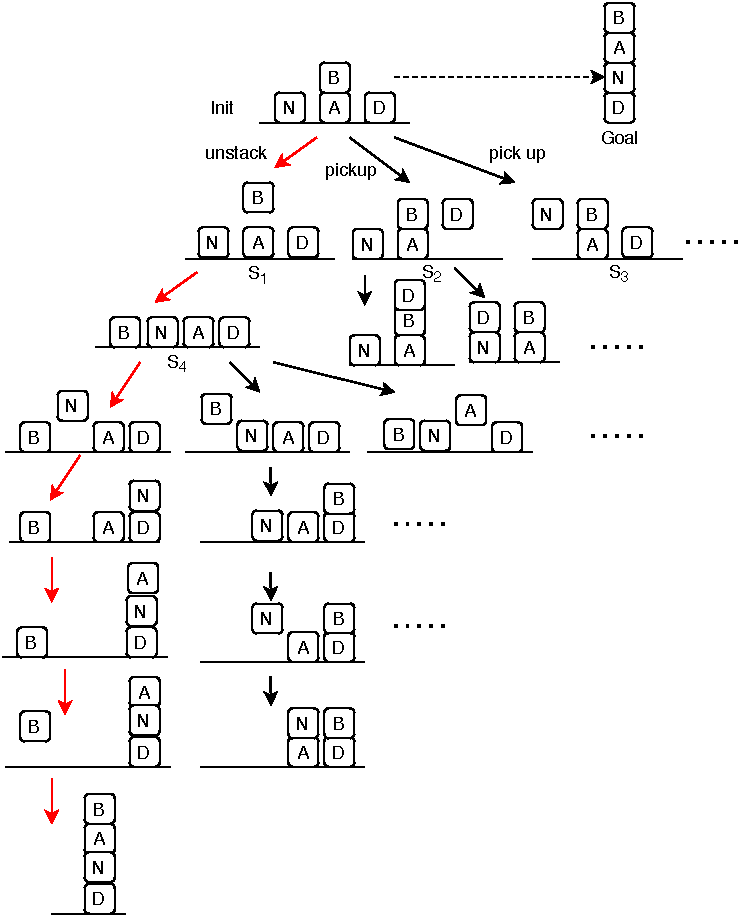
\includegraphics[width=0.6\columnwidth]{img/bw.pdf}
  \caption{Blocks Words problem as a state transition system}
  \label{fig:blockswords}
\end{figure} 

\section{Representing Classical Planning Tasks}
Although we can use the graph representation of the state transition system corresponding to a planning problem, the resulting graph can be very large and modifying this graph as new events occur in the system can become very cumbersome. In order to provide a compact representation of the transition system, \textit{states} (i.e., vertices) are represented using state variables, and actions (i.e., edges) are represented as \textit{operators} with preconditions and post-conditions specified as state variables. This way, in order to find a plan, we only need to provide the initial and goal states and use the operators to find other states as needed.

A classical planning problem can be represented using the \textbf{classical representation}, \textbf{the set-theoretic representation} or \textbf{the state-variable representation}. STRIPS \cite{fikes1971strips}, which we will use to model the domains described in this work, is an implementation of the classical representation. STRIPS uses first-order literals to describe states and actions. The set-theoretic representation is used when planning problems are solved with SAT solvers. The state-variable representation is implemented in SAS formalism \cite{backstrom91}.

In the classical representation, the world state is a set of \textbf{grounded} propositional state variables. $\Sigma$ is described using a finite set of grounded propositional state variables, which means there are only finitely many possible states. Operators that modify the world state consist of precondition propositions: propositions that must be true for the action to execute, and post-condition propositions: those will be made true as a result of the action. An \textit{action} is a ground instance of an operator. The initial state in the Blocks Words example in Figure~\ref{fig:blockswords} described in the grounded classical representation is: $\lbrace$
\texttt{ontable(N)}, \texttt{ontable(A)}, \texttt{ontable(D)}, \texttt{on(B,A)}, \texttt{clear(N)}, \texttt{clear(B)}, \texttt{clear(D)}$\rbrace$. The operator unstack is described as: \\
\textbf{operator}: \texttt{unstack (x, y)}\\[-0.5em]
\textbf{preconditions}: \texttt{(on x, y)},\texttt{(clear x)},\texttt{(handempty)},$\neg$\texttt{(equals x y)}\\[-0.5em]
\textbf{effects}: \texttt{(holding x)},\texttt{(clear y)},$\neg$\texttt{(clear x)},$\neg$\texttt{(handempty)},$\neg$\texttt{(on x, y)}

\noindent Grounding the unstack operator using blocks B and A defines the action as follows:\\
\textbf{action}: \texttt{unstack (B, A)}\\[-0.5em]
\textbf{preconditions}: \texttt{(on B, A)},\texttt{(clear B)},\texttt{(handempty)},$\neg$\texttt{(equals B A)}\\[-0.5em]
\textbf{effects}: \texttt{(holding B)},\texttt{(clear A)},$\neg$\texttt{(clear B)},$\neg$\texttt{(handempty)},$\neg$\texttt{(on B, A)}

\noindent An action is \textit{applicable} in state $s$ if $s$ satisfies the preconditions of the action. 
This means that the action's positive preconditions are  in $s$ whereas the negative preconditions are not in $s$. 
In the Blocks World example, (\texttt{unstack B A}), (\texttt{pickup D}), and (\texttt{pickup N}) are applicable in the initial state. If an action is applicable to $s$, the result of performing the action means to delete the negative propositions from the state $s$ and add the positive ones. For example, if \texttt{unstack B A} is executed in the initial state, the resulting state would be $\lbrace$ \texttt{ontable(N)}, \texttt{ontable(A)}, \texttt{ontable(D)}, $\neg$\texttt{on(B,A)}, \texttt{clear(N)}, $\neg$\texttt{clear(B)}, \texttt{clear(D)}, $\neg$(\texttt{handempty}), \texttt{clear (A)}, \texttt{holding (B)}$\rbrace$. Typically, in the classical representation, the state only explicitly contains the true propositional variables. Any propositional variable that are not included in the state is considered false.


\subsection{STRIPS Planning Task}
We now present a formal definition of a STRIPS domain and planning problem. In STRIPS, a planning task is defined using a planning domain and a planning problem.
\begin{definition}
A STRIPS planning domain is a tuple $\mathcal{D}=\langle F, Op\rangle$, where $F$ is a finite set of  state variables (predicates) and $Op$ is the set of operator schema. An operator schema $op \in Op$ is a tuple $ op = \langle Pre(op), Add(op), Del(op)\rangle$ that consists of preconditions, add and delete effects respectively, where $Pre(op)$, $Add(op)$, $Del(op)$ are all subsets of $F$. Predicates and operator schema have parameter lists and can be instantiated with objects (defined later). An instantiated operator (action) $op$ is applicable in a state $s$ if predicates in $Pre(op)$ are \textit{True} in $s$. A state transition induced by an action $op$ in a state $s$ is defined as a function $\delta$:
\begin{equation*}
\delta (s,op) = \left\{\begin{matrix}
s\setminus Del(op) \cup Add(op) & Pre(op) \subseteq s\\ 
undefined & otherwise
\end{matrix}\right.
\end{equation*}
\end{definition}

\begin{definition}
A STRIPS planning problem is a tuple $P = \langle \mathcal{O}, s_0, G\rangle$, where $\mathcal{O}$ is the set of objects. Objects can be either constant or non-constant and may have a type. Constant objects are common to all instances of the domain definition and shared by planning problems defined on that specific planning domain. Non-constant objects are unique to a specific planning problem. $s_0 \subseteq F$ is the set of propositions that are true in the initial state, $G\subseteq F$ represents the goal specification.
\end{definition}

Given a domain $\mathcal{D}$ and a planning problem $P$, an automated planner generates the planning task $\Pi=\langle \mathcal{F}, \mathcal{A}, s_0, G\rangle$, where $\mathcal{F}$ is a finite set of grounded propositions, $\mathcal{A}$ is the finite set of grounded actions instantiated from the operator schemata $Op$, $s_0$ is the grounded propositions specifying the initial state and $G$ is the grounded goal specification. Objects in $\mathcal{O}$ are used to ground $\mathcal{F}$, $\mathcal{A}$, $s_0$ and $G$. Grounding replaces the variable terms in the parameter lists of the propositions, action schema, goal specifications with constant/non-constant objects. 

\begin{definition}
A solution to $\Pi$ is a plan $\pi=\lbrace a_1, \ldots, a_k\rbrace$ of length $k$ that modifies $s_0$ into $G$ by successive execution of actions  $a_1, \ldots, a_k$ 
\end{definition}

Actions in $\pi$ may have a cost that assigns a non-negative value to the action schema defined in the STRIPS domain definition. The cost function is given as $C: Op \rightarrow \mathbb{R}^0_+$. The cost of the plan $c(\pi)$ is  $\sum(c(a_i))$. The optimal solution, the optimal plan $\pi^*$, minimizes the cost. 



\section{The Recognition Task}
Besides being able to plan, in certain cases the agent must also be able to \textit{recognize} another agent's behavior. This is specially important in the domains we are studying in this dissertation where the agent acts as an assistant to the human user.

We now extend our discussion to a multi-agent setting where, we consider at least two agents: an  acting agent $A$ and an observer agent $R$. To draw a realistic example, consider the Blocks World scenario in Figure~\ref{fig:bwpr}. Agent $A$ solves a planning task $\Pi_A=\langle \mathcal{F}_A, \mathcal{A}_A, s_{I_A}, G_A\rangle$ executes a sequence of actions $O=\lbrace$\texttt{unstack D A}, \texttt{putdown D}, \texttt{unstack R P}$\rbrace$. For simplicity let us assume that $R$ does not execute any actions, and passively observes the actions $A$ executes.

\begin{figure}[tpb]
  \centering
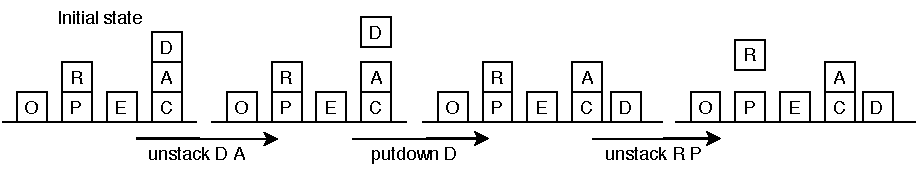
\includegraphics[width=\columnwidth]{img/bwpr.pdf}
  \caption{A recognition task}
  \label{fig:bwpr}
\end{figure}

\noindent In the recognition task, $R$ asks the question: ``What is $A$ trying to do?''. This question can be answered in three ways, leading to three types of recognition tasks:
\begin{itemize}
\item Given $O$, what is the posterior probability P($\pi$|$O$) of the complete plan $\pi$. This is the \textbf{plan recognition problem}.
\item Given $O$, what is the posterior probability P($G$|$O$) of the goal $G$, where $G \in \mathcal{G}$, a list of potential goals in the environment. This is the \textbf{goal recognition problem}
\item Given $O$, what is the posterior probability P($a$|$O$) of an activity $a$. This is the \textbf{activity recognition problem}.
\end{itemize}
\noindent Typically, $R$'s objective is to find the most likely plan, goal, activity from a set of potential plans, goals, activities in the environment. A recognition task consists of three components:
\begin{description}
\item [The environment] $E = \lbrace \Sigma, s_0, \mathcal{G}\rbrace$, is the setting in which agent $A$ acts. $s_0$ is the initial state and $\mathcal{G}$ is the set of possible goals. 
In order to perform the recognition task, the environment may produce a \textbf{plan} $\pi=\lbrace a_0, a_1, \ldots, a_n\rbrace$: a complete sequence of actions that takes agent $A$ from $s_0$ to the goal state $G$ in $\mathcal{G}$, a \textbf{history} $h=\lbrace s_0, s_1, \ldots, s_n\rbrace$: a sequence of states from $s_0$ to $G$ or an \textbf{execution} $e=\lbrace s_0, a_0, s_1, a_1, \ldots, s_n, a_n, s_{n+1}\rbrace$: a sequence of state-action transitions from $s_0$ to $G$. 
These are referred to as \textit{prefixes} in recognition. 
The recognition task example shown in Figure~\ref{fig:bwpr} considers the plan prefix. Some work in the plan recognition literature uses plan prefixes while others use the history prefixes. We will discuss work on each category. Furthermore, research has investigated recognition in both discrete and continuous domains where actions transition from one state to another via paths through the state space, rather than through discrete states (e.g., navigation domains).

\item [The acting agent (agent $A$)] must specify the assumptions made with regard to how agent $A$ acts in the environment to achieve his goal. Most of the time, recognition tasks assume that agent $A$ enters the environment and follows a plan to achieve some goal. However, $A$'s behavior may be affected by how familiar it is with the environment (e.g., are there objects that escape agent $A$'s sensors?), A's special capabilities (e.g., can he compute an optimal plan to reach $G$), and the relationship to the recognizer (e.g., does $A$ acts in such a way that his goal/plan/activity can be recognized easily or would he act to obfuscate his true goal/plan/activity?). There could be more than one agent whose goals/plans/activities we would want to recognize.
The recognition literature uses different ways to represent agent $A$ from the point of view of $R$ in the situations mentioned above. Commonly used representations are \textbf{plan libraries} and \textbf{domain theories}.

\item [The recognition system (agent $R$)] When defining a recognition problem, the final component is the specification of the recognizer. Here, we need to define several components: 
\begin{itemize}
\item the observability: how does agent $R$, perceive agent $A$'s behavior (e.g., is there any noise in the observations? Are there any actions/states $R$ can not perceive?)
\item the objective: what does $R$ need to do? (e.g., recognize $A$'s goal/plan/activity as soon as possible? is the recognition online or offline?)
\item the possible interventions: can $R$ interact with $A$ or affect its behavior? (e.g., provoke $A$ to change its course during execution, modify $\Sigma$ to help recognition)
\end{itemize}

\end{description}

We now present a framework, within which we discuss selected prior work from goal and plan recognition. We set up the framework along three dimensions:
\begin{description}
\item [single vs. multi actor] In the single actor case, $R$ makes observations of a single actor agent to recognize the goal/plan of that agent. In the multi-agent case, the observations originate from many agents. Furthermore, the goals pursued by the agents in the system may be a complex goal. For example consider an agent $X$ assisting two other agents ($Y$ and $Z$) pursuing two different goals $G_Y$, $G_Z$ respectively. $X$'s goal $G_X$ an be defined as $G_Y \cup G_Z$. Thus, in a multi-agent system $R$ may have to recognize complex goals as above, instead of one goal shared by all agents.
\item [online vs. offline] In online recognition, the observations are incrementally revealed to $R$. Recognition is performed based on the observations revealed thus far (i.e., a partial observation trace). In offline recognition, the complete observation trace is available to $R$ up front and recognition is performed accounting for information available from the full observation trace.

\item [the recognizer's interaction with the actor] In this dimension we discuss different ways $R$ can communicate with $A$ during the recognition process. In most related work, the recognition task terminates when $R$ identifies what $A$'s goal or plan is. Interaction is an extension of the typical recognition problem. Some work on interaction suggests modifying the environment (e.g., blocking some actions $A$ could otherwise have executed) to facilitate early recognition of $A$'s goals/plans. Others propose question-answering approach where $R$ queries $A$ about his plans/goals and reasoning about information acquired from the queries.
\end{description}

\noindent Within the three-dimensional framework, for each related work shown in Table~\ref{tab:relatedwork} we also discuss the properties of the \textbf{environment}, the \textbf{acting} agent and the \textbf{recognizer} agent around which the recognition tasks are modeled. Our discussion on related work also extends to work that are not listed in Table~\ref{tab:relatedwork}. We do this mainly to draw comparisons between how the work listed in Table~\ref{tab:relatedwork} improves/extends other (earlier) noteworthy plan and goal recognition work.

\begin{table}[tpb]
\caption{Fitting related work to the analysis framework}
\label{tab:relatedwork}
\resizebox{\columnwidth}{!}{
\begin{tabular}{|l|c|c|c|c|c|c|}
\hline
\multirow{2}{*}{Related Work} & \multicolumn{3}{c|}{Plan Recognition}       & \multicolumn{3}{c|}{Goal Recognition}       \\ \cline{2-7} 
                              & Single/Multi & Online/Offline & Interaction & Single/Multi & Online/Offline & Interaction \\ \hline
Ramirez et al. 2009       &        &         &      & Single & Offline & None \\
Ramirez et al. 2010       & Single & Offline & None &        &         &      \\
Sohrabi et al. 2016  	  & Single & Offline & None &        &         &      \\
Vattam et al. 2015        & Single & Offline & None & 
&  		&  \\
Vered et al. 2017 &        &         &      & Single & Online  & None \\
Boddy et al. 2005      & Single & Offline & None &        &         &      \\
Keren et al. 2014       &        &         &      & Single & Offline & Yes  \\
Pozanco et al. 2018     &        &         &      & Muti   & Online  & Yes  \\
Mirsky et al. 2016      &        &         &      & Single & Online  & Yes  \\ 
Shvo et al. 2018  	 & Multi  & Offline & None &        &         &      \\ \hline
\end{tabular}
}%
\end{table}

\section{Plan Recognition}
The plan recognition problem is to \textit{take as input a sequence of actions performed by an actor and to infer the  goal pursued by the actor and also to organize the action sequnce in terms of a plan structure} \cite{schmidt1978plan}. This requires some method to represent how the actor would act in the environment. Recognition solutions that use automated planning represent the actor's behavior as a planning problem focusing on the fact that the actor moves from state to state and changes the environment to achieve some goal. The solutions that use parsing assume that plans are constructed as a hierarchy in the actor's mind.

Early solutions to the plan recognition problem require that the part of a plan given as input to the recognizer be matched to a repository of example plans. This repository is referred to as a \textit{plan library}. The plan library represents possible plans the acting agent may be trying to execute in the environment $E$. In the plan recognition literature, several methods have been proposed as representation models of the plan library.

\subsection{Plan Recognition with Plan Library Representations}
Many plan library representations use graphs to represent a possible plan that will likely execute in the environment. 
In The Generalized Plan Recognition \cite{kautz1986generalized}, the recognition problem is defined as identifying a \textit{minimal set of top-level actions sufficient to explain the set of observed actions}. 
Here, the plans are modeled in a graph. 
The nodes of the graph represent the actions. 
The graph has two types of edges: action specialization (between top-level actions) and action decomposition into sub-actions.
The authors use a cooking domain as the example and define the top level actions and recursively decompose those actions until no further specializations can be made. 
Lower level actions in the plan graph \textit{logically imply} the higher level actions. 
For example the top level action ``PrepareMeal'' specialized into ``MakePastaDish'', specialized into ``MakeFettuciniMarinara'', decomposed into two leaf-level actions ``MakeFettucini'' and ``MakeMarinara''. The implication relationships are derived from bottom to top. Given this representation of the plan library, the plan recognition task becomes the minimum vetex cover problem of the graph. This recognition problem contains one actor and one recognizer.

Geib and Goldman represent the plan library for a cyber security domain as partially ordered AND/OR trees \cite{GeibGoldman09}. 
Their representation also assumes that the tasks the actor agent is trying to complete in the domain are hierarchical. 
AND nodes in the graph require that all sub-tasks be achieved before completing the parent task. 
OR nodes represent instances where the actor agent may choose between alternatives to complete the parent task. 
The subtasks themselves may further be represented as AND/OR (sub) trees. The root of the tree is the goal. Plans are derived from traversing to leaves from the root of the tree. The plan library is augmented with probabilities (i.e. prior probabilities of root goals, OR tree choice probabilities etc.).
Then, in order to recognize the actor's plan, the recognizer needs to compute the probability of an explanation (plan) given the observations (i.e. P$(\pi|O)$). 
Specifically, the recognizer needs to derive a probability distribution over a set of likely explanation plans. 
To extract the likely explanation plans, the authors define a grammar to parse the AND/OR trees and generatively build the explanations by starting off with a ``guess'' and refining it as more observations arrive. 
The actor in this work is hostile. This means that the actor does not want the recognizer to find out his plan and he will hide some actions. 
This causes the recognizer to deal with partial observability when computing P$(\pi|O)$. 
This topic is left for future work.

\subsubsection{Plan Libraries: What is the Problem Anyway?}
One issue with using plan libraries is that it is difficult to ensure the completeness of the plan library. It is unrealistic to encode \textit{all} possible plans for a given planning problem into a plan library. However, the system must still be able to reason about new but correct plans the agent may pursue. Cohen et al. propose a new approach for updating a plan library with new plans \cite{spencer1993}.

Another issue with using plan libraries for recognition is the noise in the input observations. A key assumption in the library based solution is that the observations must be able to associate with one or more recipes in the library, and the partial plan inferred for the agent must reflect the agent's intended goal or plan. Noise in the observation trace may occur from missing actions (e.g., noisy sensors, agent deliberately hiding observations, etc.) or exogenous events that occur in the environment that have nothing to do with the agent's true goal/plan. Rich et al. proposes  a method to enable the plan library to incrementally relax the constraints on recipes before declaring that the recipe is not found \cite{rich2001collagen}. They use a \textit{focus stack}, that maintains a set of annotated goals that are being pursued. The goals are removed from the tack only when the goal is complete.

\noindent\textbf{Vattam et al. 2015 - Case-based Plan Recognition}

The case-based plan recognition \cite{vattam2015case} relaxes the error-free requirement of the observations in plan recognition problems and introduces a recognition algorithm that can handle \textbf{missing} and \textbf{misclassified} actions in the observation trace. This problem is also modeled with a single actor and a single passive recognizer agent and assumes that there exists a plan library consisting of a set of \textit{cases}. A case consists of a planning problem and a fully grounded solution plan to this planning problem. Given a subsequence of actions, the algorithm needs to address two requirements: (1) matching the incoming sequence to the stored cases to retrieve candidate plans and (2) evaluating the retrieved cases to identify the top-ranked candidate plan (i.e., recognize plan).

Cases are stored using labeled, directed graph called an \textit{action sequence graph}. 
This data structure facilitates comparisons between incoming observations and the stored plans using similarity metrics derived from the graph topology. In order to account for errors in the observations, plans are represented as a sequence of action-state pairs: $\mathbb{S}=\langle (null,s_0), (a_1, s_1), \ldots, (a_g,s_g)\rangle$. $s_0$ is the initial state and $s_g$ satisfies the goal $g$. This is in contrast to the typical representation of a plan, which is a sequence of actions. Given an action-state pair $(a,s)_k \in \mathbb{S}$, they first produce the predicate encoding graph $\epsilon$, a labeled, directed graph such that the vertices encode the action $a$, the state fact $s$ and the corresponding parameters of $a$ and $s$. Then two types of edges are created for both action and the state fact that connect the predicate and the first parameter and an edge for each pair of parameters in the predicate's parameter list. An edge is labeled based on the two nodes that it connects. Once each action-state pair $\in \mathbb{S}$ generates its own $\epsilon$, the action sequence graph is generated by their union.

Given the action sequence graph of a sequence of action-state pairs and a plan library consisting of action sequence graphs, candidate plans are retrieved by evaluating the structural similarity between them. This work proposes two graph based similarity metrics (degree sequences similarity metric, combined similarity metric), which can approximate the \textit{maximum common subgraph} to match the incoming graph to the graphs in the library. Then the top k graphs based on the approximated metric values are selected as the recognized plans.

\noindent\textbf{Constraints in the Approach}\\
This approach is tested on the Blocksworld benchmark domain. The plan library is small and errors to the observation sequences are introduced systematically, rather than attempting to simulate realistic conditions. In the application domains we are studying for this research, the human users interact with the recognition system, which means that errors may appear in the observation trace in an ad-hoc manner. Furthermore, the user (due to partial visibility/lack of knowledge) may not realize the action they take is incorrect and do it anyway. This requires that the recognition system be able to ``evaluate'' partial observation sequences based on the extent to which it helps task completion while avoiding errors.

Next, we introduce a second approach for solving plan recognition problem, which does not require the existence of a plan library.


\subsection{Solving the Plan Recognition Problem with Domain Theory}
\label{sec:prpdomain}
\noindent\textbf{Ramirez et al. 2010 - Probabilistic Plan Recognition}

Ramirez and Geffner proposed a plan recognition solution that does not rely on defining a plan library \cite{ramirez2010probabilistic}. 
Their approach has the advantage of being able to exploit automated planners to sample the plan space to find plans that are compatible with the observations. 
This allows the recognition problem to scale up well to handle domains with a large number of actions and state variable predicates.

The environment $E$ discussed in this solution consists of one actor agent and one recognizer. The actor is not executing an optimal plan. The recognizer passively observes the actions executed by the actor. 
Figure~\ref{fig:prp} illustrates a grid based plan recognition task, where an actor moves through a $8\times5$ grid. 
The actor initially is the position indicated by \textbf{I}. 
The actor attempts to accomplish one of the possible set of goals $\lbrace$A, B, C, D$\rbrace$, by moving either horizontally, vertically, or diagonally. 
Using PDDL, we can represent the possible set of goals $\mathcal{G}=\lbrace$ (\texttt{at A}), (\texttt{at B}), (\texttt{at C}), (\texttt{at D})$\rbrace$. \textbf{F} is the current position of the actor. 
Assume that horizontal and vertical moves have cost of 1, and diagonal move has a cost of $\sqrt{2}$. 
The arrows show the path the actor has taken, which consists of three moves (2 vertical and 1 diagonal). The recognizer asks the question, ``\textit{Given the three moves (up,up,diagonal) what is the actor's most likely goal}?'' Formally, the plan recognition problem $\mathcal{R}$ is a tuple such that $\mathcal{R}=\langle \mathcal{F}, \mathcal{A}, s_0, \mathcal{G}, O, PROB\rangle$, where $\mathcal{F}$ is the set of state variable predicates, $\mathcal{A}$ is the set of actions, $s_0$ is the initial state, $\mathcal{G}$ is the set of possible goals, $O$ is an observation sequence $O=\lbrace o_1,\ldots o_m\rbrace$ and $PROB$ is a prior probability distribution over $\mathcal{G}$. 
In this work, each $o_i\in O$ is an action in $\mathcal{A}$.
Note that $\mathcal{F}, \mathcal{A}, s_0$ are collectively known as the \textit{planning domain theory}.

\begin{figure}[tbp]
  \centering
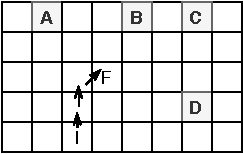
\includegraphics[width=0.5\columnwidth]{img/rg.pdf}
  \caption{The plan recognition problem}
  \label{fig:prp}
\end{figure}

Ramirez and Geffner provides a solution to the recognizer's question by accounting for the cost differences of two types of plans for each goal: (1) plans that reach a goal while going through the observations and (2) plans that reach a goal without going through the observations. Formally,
$\forall g \in \mathcal{G}: \Delta_{g} = C_g(O) - C_g(\overline{\rm O})$, where $\Delta$ refers to the cost difference, $C_g(O)$ refers to the cost of the plan that reaches goal $g$ going through $O$ and $C_g(\overline{\rm O})$ is the cost of the plan that reaches the goal without going through $O$. In the example in Figure~\ref{fig:prp}, when the agent is (\texttt{at F}),\\
$\Delta_{(at A)}= (2+3\sqrt{2}) - (3+\sqrt{2})=1.8$\\
$\Delta_{(at B)}= (3+2\sqrt{2}) - (2+2\sqrt{2})=1$\\
$\Delta_{(at C)}= (6+2\sqrt{2}) - (4\sqrt{2})=3.2$\\
$\Delta_{(at D)}= (4+2\sqrt{2}) - (3+\sqrt{2})=2.4$\\
This indicates that from the given observations, (\texttt{at B}) has the least cost difference. What does that mean? 
According to the $\Delta_g$ formula, if for a specific goal, if $C_g(O)$ is greater, it follows that $\overline{\rm O}$ is more likely than $O$ (because the rational actor agent would follow the lower cost plan). 
Putting it differently, smaller $\Delta$ means that cost of $\overline{\rm O}$ plan is greater, thus the agent is likely following the plan that is aligned with the observations. 
Therefore, given the observations, the most likely goal would be the one that has the least cost difference. 
The solution to the plan recognition problem is expressed as the subset of goals $g\in \mathcal{G}$ such that the \textit{optimal} plan for $g$ satisfies the observation sequence $O$.

How does the recognizer produce plans that are compatible with the observations? 
For this, Ramirez and Geffner use a technique called ``\textit{Compiling Observations Away}''. When the observations are compiled into the domain theory, it forces the automated planner to search for solutions that already contain the observations. 
They transform the original domain (defined in STRIPS) $D$ into a domain $D^\prime$ given the observations $O$. The new domain has the same initial state and actions as $D$. 
However, new state variable predicates are added to $D^\prime$ such that if an action $a$ is in $O$, it's definition in the domain gets added an extra state variable predicate to its post-conditions. 
This modification is done only if $a$ is the first observation in $O$. 
If there is an action $b \in O$ that immediately comes before $a$, then the preconditions of action $a$ gets added a new state variable predicate (that is already in the post conditions of $b$) and post conditions of action $a$ gets added a second new state variable predicate.

Once these modifications are done to the domain definition $D^\prime$, automated planners can be used to find plans that are compatible with the observations. $D$ is used to find plans that are not compatible with the observations. Then, to do the recognition task for each $g\in \mathcal{G}$ they compute the posterior probabilities $P(g|O) \cong \alpha P(O|g) P(g) $, where $P(g)$ is the prior probability for $g$ given as input to the recognition task and $\alpha$ is the normalizing constant. Ramirez and Geffner characterize the likelihood $P(O|g)$ as a Boltzmann distribution $P(O|g)=\frac{e^{-\beta\Delta_g}}{1+e^{-\beta\Delta_g}}$ where $\beta$ is a positive constant and $\Delta_g$ is the cost difference between observation compatible and not compatible plans for goal $g$.

\noindent\textbf{Constraints in the Approach}\\
In order to compute the posterior probabilities over the likely goals, the planner has to be invoked twice: once to find the observation compatible plans and once to find the plans that are not compatible. 
This may be costly for large problems and plan recognition in real time (i.e., when observations arrive incrementally). 
Furthermore, for the two costs to be different (and enable the recognizer to correctly identify the actor's goal) the observations must contain action landmarks for the goal we want to identify.
Landmarks are state predicates that must be true in any valid plan to reach the goal \cite{hoffman2004lm}.
Action landmarks contain the landmarks as their post-conditions. 
If the observed action is an action landmark for $g$, then $C_g{(\overline{\rm O})}$ will be higher and as a result $P(g|O)$ will be higher. If there are many ways to reach $g$ (i.e., no action landmarks) then the cost difference $C_g(O) - C_g{(\overline{\rm O})}$ will not be significantly different and as a result, it will be harder for the recognizer to identify the correct goal. 
A solution that address these constraints is proposed by E-Martin et al., which calculates the \textit{interaction} of two or more actions \cite{yolanda2015} using the \textbf{plan graph} representation of the planning task  \cite{blum1997fast}. 
They first define the cost of two proposition/actions to be established together (\textit{cost interaction}). 
This cost is propagated through the plan graph starting from the initial state until the goal states are achieved. 
The cost of achieving the goal is the sum of interactions between propositions and the costs of actions required to achieve that goal.
Like Ramirez's solution, this work also assumes that the observations are not noisy but may be incomplete.

In certain problems, it maybe difficult to provide reasonable prior probabilities for the likely goals. This is specially true in the kinds of planning domains we are working on in this research, where certain facts about the domain are hidden to the actor and the absence of complete knowledge may enable some unintended goals, regardless of their priors. For example, consider a human user unwittingly falling victim to a phishing scam because he can not recognize phishing web sites from the safe ones.

Furthermore, in certain cases the recognizer may need to recognize the actor's plan before all the observations are made available. This is also an important requirement in the domains we are studying in this research, where an agent needs to assist human users avoid certain undesirable consequences before the human user's task is completed. This requires that recognition needs to happen as observations are made available incrementally. We will discuss some recent work in online recognition in the following sections.

\noindent\textbf{Sohrabi et al. 2016 - Plan Recognition with Unreliable Observations}\\
The recognition task is similar to the probabilistic plan recognition problem proposed by Ramirez and Geffner, where a recognizer receives an observation trace of the actor's agent's behavior and attempts to identify what the actor's plan is. They also use the ``\textit{Compiling Observations Away}'' theory to generate a solution to the plan recognition problem. Sohrabi et al. propose several extensions to prior work where (1) the recognition system can now handle noisy or missing observations and (2) address observations over state variables. Further, the recognizer can identify the actor's plan and goals.

This work defines a \textbf{noisy} observation as an action that can not be explained by actions of a plan for a particular goal. \textbf{Missing} observation is an action that should have been in the observation trace but have not. When the observations are unreliable, the cost difference $C_g(O) - C_g{(\overline{\rm O})}$ will be large and as a result it will underestimate $P(g|O)$. This is because with noise in the trace, either the plan that is compatible with $O$ will have a higher cost than the plan that is not compatible with $O$ or the planner may not be able to find an observation compatible plan. To remedy this situation, they propose a new approach to ``\textit{Compiling Observations Away}'' that modifies the planning domain to include action costs; specifically penalties for noisy/missing observations.

In Ramirez and Geffner's work, the observations are presented as actual actions as defined in the domain theory. Shorabi et al. argue that in realistic examples, it may be difficult for the recognizer to observe the action itself, but he may be able to observe the effect of the action in the state. Therefore, they define the observations over state variables instead of actions. When  ``\textit{Compiling Observations Away}'', they augment the domain $D$ with special ``discard'' and ``explain'' actions. This classification helps to identify noisy observations that must be discarded. The definition for the plan recognition problem $\mathcal{R}$ closely follows from Ramirez and Geffner's definition, where $\mathcal{R}=\langle \mathcal{F}, \mathcal{A}, s_0, \mathcal{G}, O, PROB\rangle$. However, $O$ is now a sequence of states, instead of actions. Recall that the domain theory $D=\langle \mathcal{F}, \mathcal{A}, s_0 \rangle$. The augmented domain theory $D^\prime=\langle \mathcal{F}^\prime, \mathcal{A}^\prime, {s_0}^\prime\rangle$. $\mathcal{F}^\prime$ contains state variable predicates from $D$ plus the new predicates  $done, l_{o_0}$ to signal that the goal state is complete and to indicate the start of the $O$ respectively. 
In addition  $\mathcal{F}^\prime$ has a set of special predicates $l_{o_i}$ for each observation $o_i$ indicating whether the observation was discarded or explained. 
The special predicates ensure the total order of observations is maintained when the new actions are executed. 
${s_0}^\prime$ is equal to $s_0$ and has the additional predicate $l_{o_0}$. Goal $G^\prime \in \mathcal{G}$ are expressed such that $G^\prime = \lbrace done, l_{o_m}\rbrace$, where $l_{o_m}$ is the last observation. There are four types of actions in $\mathcal{A^\prime}$, each having costs associated with them \textbf{goal} action, \textbf{discard} action, \textbf{explain} action and original actions from $\mathcal{A}$. The \textit{goal action} has preconditions equal to the goal state, postcondition equal to $done$ and cost = 0. The \textit{discard action} is added when the observed state is false in the current state (i.e., observation not explained). As the post condition, the discard action adds the special predicate $l_{o_i}$ and removes the special predicate added by previous observation $l_{o_{i-i}}$. Discard action cost = $b_2$ (a application specific weight). The \textit{explain action} is added when the observed state is true in the current state. The post condition is similar to the discard action. The explain action has cost = 0. The \textit{original action} has the same pre/post conditions from the original definition $\mathcal{A}$. However, it is now assigned a new cost, which adds a penalty proportionate to the number of missing observations. The plans derived from the augmented domain theory $D^\prime$, now reflect penalties to missing and unexplained observations.

The recognition task is performed by deriving posterior plan probabilities P($\pi|O$) and posterior goal probabilities P($G|O$) following the same process as Ramirez and Geffner. 
\begin{itemize}
\item $P(\pi|O) = \beta P(O|\pi)P(\pi|G)P(G)$
\item $P(G|O) = \beta P(O|G)P(G) = \beta \sum_{\pi \in \Pi}P(\pi|O)P(G)$
\end{itemize}
$P(G)$ is an input to the recognition problem as $PROB$. Note that, now $P(G|O)$ depends on $P(O|\pi)P(\pi|G)$. Sohrabi et al. approximates this value such that $P(O|\pi)P(\pi|G) \approx 1- \frac{\beta V(\pi)}{\sum_{\pi^\prime \in \Pi}V(\pi^\prime)}$, where $V(\pi)$ is a weighted cost factor that accounts for noisy and missing observations in a plan $\pi$ for goal $G$ that satisfies $O$.  The term $\sum_{\pi^\prime \in \Pi}V(\pi^\prime)$ is computed from the sampled plans that are derived from the augmented domain theory $D^\prime$ using Top-K planner \cite{riabov2014}, which finds k-best plans and using diverse plans. The recognized goal/plan is the goal/plan that has the highest posterior probability from the set of most likely goals/plans.

\noindent\textbf{Constraints in the Approach}\\
Similar to Ramirez and Geffner's work, this solution for plan and goal recognition relies on being able to provide the goal priors as an input to the algorithm. Furthermore, the observations (although given as a sequence of states) need to be provided to the algorithm up front. For the assistive agent we are designing for human users, the recognition process needs to be separated from these constraints.

\subsection{Shvo et al. 2018 - Multi-agent Plan Recognition}
So far, we have only discussed plan recognition in situations where there is one actor and one recognizer. An extension to this paradigm is proposed in work by Shvo et al. \citeyear{shvo2018}, where the Multi-agent Plan Recognition problem (MAPR) is introduced. In MAPR the recognizer infers the goals and plans of multiple agents. The observations given to the recognizer originates from many agents. MAPR has interesting applications in multiple real domains such as intrusion detection, surveillance and so on.

When performing MAPR, the recognizer takes into account different capabilities of the agents in the domain. In addition, this work further considers actions taking some time to finish executing (durative actions). Similar to the work by Shorabi et al., observations are processed as states and not as actions. Furthermore, observations may be unreliable (i.e., contains missing/unexplainable observations). This solution to MAPR problem also builds on the plan recognition approach proposed by Ramirez and Geffner that proposes modifications to the domain theory to recognize goals/plans using automated planners. In the first step, the multi-agent aspect is compiled away into the domain theory. When there are many agents in the environment having different actions that they can execute, some actions can be executed concurrently, while others can not. They use temporal nature of actions to establish ordering constraints on the actions.  Two special state predicates are defined for actions that operate as \textit{action delimiters}: ``start'' and ``end'', which specify the pre and post conditions to the temporal action respectively. Additionally, they also define an overall precondition to the temporal action, which must hold true in every state between the ``start'' and ``end'' states. When actions are temporal, the solution plan is a sequence of action-time pairs showing actions that can execute at the same time when they are applicable.  Use of temporal actions allows concurrency of the agent's own actions as well as actions of different agents. Now, in order to compile away the multi-agent aspect, they define a privacy model for the agents when executing the temporal (and perhaps shared) actions. Action $a$ can be executed by agent $i$ if and only if $a$ is private to agent $i$ or is public to all agents. This is done by introducing special predicates to track the ownership (i.e., which agent, what objects) of state variables when a temporal action is being executed. This privacy model is added to the initial state of the planning problem. The second step is ``\textit{Compiling Observations Away}''. Here, they follow the same process as Sohrabi et al. 2016 to ``\textit{Compiling Observations Away}'' for missing and noisy observations. Then, the plan recognition problem becomes finding the posterior probabilities of plans P($\pi|O$) and  goals P($G|O$). Because the domain theory now has temporal actions, it is possible to use temporal planners to find sample solution plans.

\noindent\textbf{Constraints in the Approach}\\
The proposed approach is only evaluated for a case where the agents pursue one common goal. The assistive recognizer agent we are presenting in our research is an extension to this work. When different agents pursue different and competing goals, and when the recognizer is expected to assist one agent in the environment it needs to consider how likely the goal of the agent (who is being helped) will be threatened by competing agent(s) actions. The recognizer agent must be  able to complete recognition \textit{in time} to identify when a partial plan that seems to be helpful can be subverted by a competing agent during execution and alert the agent accordingly.



\subsection{Planning as a Tool to Model User Behavior in Cyber-security}
Cyber-security domain offers a lot of promise to study behavior both as normal users and as adversaries in automated planning. Behavioral Adversary Modeling System (BAMS) \cite{boddy2005course} uses automated planning to help computer network administrators in analyzing vulnerabilities in their system against various kinds of attacks. BAMS takes into account the properties of an adversary and produces plans that lead to system exploits that also coincides with the adversary model. While this work does not directly apply to plan recognition at its core, it illustrates a use case where classical planning can be used to design assistive systems targeted towards human end users.

This work models network vulnerabilities of a document management system as a planning problem and integrates a predictive behavior model of an adversary (who is a malicious insider) so that network administrators can concentrate on hardening the system in places where exploits are most likely and result of the exploit will be most costly. The network security planning domain contains objects such as email messages, files, hosts, user identifiers etc. and has 124 predicates to represents facts about the environment, status of tiles, capabilities, vulnerabilities of programs, knowledge possessed by users etc. Actions are represented in STRIPS with parameters, pre and post conditions. The domain has 56 actions that capture system events such as document accesses, user group modifications etc. The adversary's objectives are specified in the planning problem as goals. They use an off-the-shelf planner Metric-FF  \cite{hoffman2003ff} to find possible plans of the adversary. A graphical user interface allows end-users (i.e., network administrators) to configure problem specifications (hosts in the system, access control rules etc) and the attacker's properties (skills/tools he has) without having to encode them in PDDL.

The authors highlight several issues in modeling expressive scenarios in PDDL. 
The first constraint is the difference between the level of detail that is required in the domain and what can be modeled in the planning language. If the representation is too detailed, the resulting plans will be uninteresting and difficult for the users to extract information. Furthermore, developing and maintaining these highly descriptive domains will be a difficult task requiring expert knowledge. The second constraint is providing the plans generated by the automated planner to end-users in a natural representation. PDDL plans are not naturally comprehensible to end-users. The authors propose an encoding scheme for the PDDL actions and providing explanatory texts to capture state transitions that take place within the solution plan.

In this dissertation, we take a step toward designing assistive systems using automated planning to help human end users, who are non-experts (e.g., home users). 
Home users are specially vulnerable to undesirable consequences because they lack the know-how to recognize risky situations in advance.
A previous study \cite{byrne2016} showed that home users pay more attention to the benefits of the activities than the risk; they have goals that they want/need to achieve and are willing to take the risk to achieve them. Many triggering actions may be normal
activities (e.g., reading email, clicking on links) with the user more focused on the goal than on the risk. Thus, the undesirable consequence recognition problem needs to take into account the user’s intention as well as the undesirable consequence.

Howe et al. \citeyear{howe2012psychology} observed that most studies that look into computer security practices of users relying on self reported surveys suffered from issues such as respondent bias, socially desirable responding and peer perception.
The authors posited that experiments based on simulation, which place the participant in the actual situation that is monitored can help reduce such issues and also be leveraged to assess the emotional reactions of users to interventions and warnings.

The Intervention Problem can be directly applied in the cyber-security domain.
An attacker attempting trick the user into compromising his security/privacy during day-to-day computing tasks fits the model of the competitor we discussed in this work.
The attacker creates opportunities for phishing and malware attacks by making them to appear as common harmless tasks such as email and installing software. 
Unable to recognize these attacks in advance, the user becomes an unwitting accomplice to security breaches.


\section{Goal Recognition}
Similar to plan recognition, early goal recognition solutions involved using plan libraries. Lesh and Etzioni \citeyear{lesh1996} use a plan library based approach for goal recognition. Here, they use a data structure called a \textit{consistency graph}, which is a directed graph with actions, action schema, and goals as nodes. There is an edge between two nodes if there is a \textit{consistent} plan that supports the two nodes for some goal. Their approach to recognizing an actor's goal rely on quickly determining if a goal is inconsistent with the observed actions. Informally, the recognizer needs to conclude that the actor could not possibly have executed the observed actions as a part of a plan to satisfy the goal. This requires the recognizer to reason about \textbf{all} plans for each candidate goal. Consistency graph is an efficient way to represent planning problems and reason about them tractably.

Similar to the plan recognition problem, the goal recognizer takes as input a set of likely goals, a sequence of actions executed by the actor, actor's beliefs and a model of action schema that can be executed in the domain. The solution to the goal recognition problem is a subset of the goal schema such that, for every element in the subset, there exists a plan that achieves that goal. In order to find this goal schema subset, they first build the consistency graph. Then they gradually remove elements (action schemas/goal schemas) following a predefined rule set, which recognizes elements in the graph that are not in any consistent plan without violating the graph correctness.

Actions are removed from the consistency graph when the observed action is not consistent with other actions in the plan or the goal. This rule is sensitive to noisy observations. Oftentimes, human users do not take actions to achieve a goal in a rigid sequence. For example, they may try a few options before settling into one plan or they could just be \textit{exploring} the domain. This is specially true in the kinds of domains we are investigating in this research: cyber-security and Rush Hour. Actions generated in these type of situations may eventually be removed from the graph, which results in the recognizer failing to identify the actor's goal.

\subsection{Ramirez et al. 2009 - Plan Recognition as Planning}
This work is the precursor to the probabilistic plan recognition work proposed by Ramirez and Geffner that we discussed in plan recognition related work. There are many similarities between plan recognition as planning \cite{ramirez2009plan} and probabilistic plan recognition. As stated in the previous work by the same researchers, the environment $E$ and the recognizer's problem are defined the same. They both use the domain theory to generate two types of plans to find the most likely goal: (1) one that is compatible with observations and (2) one that is not compatible with observations.
The key differences are the assumption that the actor is only executing optimal plans and the approach they use to compile the observations away. The ``\textit{Compiling Observations Away}'' technique used in this work to modify the original domain theory $D$ into a new domain theory $D^\prime$ by adding new action definitions and predicates corresponding to the observations.

Let us define $D = \lbrace \mathcal{F}, \mathcal{A}, s_0 \rbrace$ for plan recognition problem illustrated in Figure~\ref{fig:prp}. $\mathcal{F}= \lbrace (at\:x), (adj\:x,\:y), L1\_1, L1\_2, \ldots, L8\_5\rbrace$, which indicates that the actor is at location $x$ and location $x$ is adjacent to location $y$ respectively. Predicates $L1\_1$ etc. refer to the cells on the grid, corresponding to the row and the column numbers of the cell. $\mathcal{A}= \lbrace move(x,y)\rbrace$, which indicates that the agent can move from location $x$ to location $y$. Preconditions of the move operation $pre(move)=\lbrace (at\:x)  \land  (adj\:x,\:y) \rbrace$. Post-conditions for the move operation $add(move)=\lbrace (at\:y) \rbrace$, $del(move)=\lbrace (at\:x) \rbrace$. The initial state $s_0=\lbrace (at\:L5\_3)\rbrace$. Let us assume the recognizer gets the observation trace $O=\lbrace move(L5\_3, L4\_3)\rbrace$, which indicates that the actor has moved up one cell from the initial position.

\sloppy
If we are to apply the \textit{Compiling Observations Away} theory proposed by Ramirez and Geffner to transform $D$ to $D^\prime=\lbrace \mathcal{F}^\prime, \mathcal{A}^\prime, {s_0}^\prime\rbrace$ adds one new state variable predicate such that $\mathcal{F}^\prime=\mathcal{F}\cup\lbrace p_{move(L5\_3, L4\_3)}\rbrace$ and one new action such that $\mathcal{A}^\prime=\mathcal{A}\cup\lbrace ob_{move(L5\_3, L4\_3)}\rbrace$. The new state variable predicate indicates that the an observation has occurred in the environment (in this case, move up). The new action is fully grounded and defined below.\\
\textbf{operator:} $\texttt{ob}_{\texttt{move}(L5\_3, L4\_3)}$\\
\textbf{preconditions:} $\lbrace$ (\texttt{at}$\:L5\_3$) $\land$  (\texttt{adj}$\:\:L5\_3$,$\:L4\_3$) $\rbrace$ \\
\textbf{postconditions:} $\lbrace$ $\neg$ (\texttt{at}$\:L5\_3$) $\land $ (\texttt{at}$\:L4\_3$) $\land$ $\texttt{p}_{\texttt{move}(L5\_3, L4\_3)}$ $\rbrace$\\
Comparing this to the compilation proposed in probabilistic plan recognition, the probabilistic method does not add any new action definitions to the domain theory. Instead, only the new state variable predicates are added into existing action definitions. In order to force the planner (an optimal planner in this case) to find solutions that are optimal in number of moves and also contains actions in the observations, the goals $\mathcal{G}$ are also modified to reflect the effects of the observation. For example, the goal $g \in \mathcal{G}$ such that $g=\lbrace$(\texttt{at}$\:L1\_2$)$\rbrace$ is modified to  $g^\prime=\lbrace$(\texttt{at}$\:L1\_2$)$ \:\land\: \texttt{p}_{\texttt{move}(L5\_3, L4\_3)}\rbrace$. The process of adding new state variable predicates and new actions is repeated for all actions in the observation trace. All goals in the candidate goal set are also modified accordingly. The likely goal given observations ($P(g|O)$) is found by the same calculation as the probabilistic plan recognition by taking the cost difference between optimal plans that contain the observations and optimal plans that do not contain the observations.


\noindent\textbf{Constraints in the Approach}\\
This work also has the same constraints as the probabilistic plan recognition, in that the goals are recognized when all the observations are available and the difficulty in specifying the goal priors. Plan intervention requires us to identify undesirable consequences before the task is completed. It follows that the offline model of recognition is not suitable for plan intervention. However, we will use the plan recognition with ``\textit{Compiling Observations Away}'' theory to benchmark our initial plan intervention solutions.


\subsection{Vered et al. 2017 - Online Goal Recognition in Continuous Domains}
So far, the goal and plan recognition problems we have discussed in this chapter assume the actor and the recognizer are in a discrete domain and the observations are discrete. Online goal recognition \cite{vered2017} extends the recognition problem to continuous domains. For example, in robot motion planning, we can define a simple domain as the space of possible positions for a robot. This definition can further be extended to define higher order dimensions such as angle, velocity etc. Further, the recognition is online, which means that the recognition problem must be solved for every new observation when they are revealed. The recognizer receives observations of the actor's position in the same n-dimensional space (e.g., a point or a trajectory). The recognition problem them becomes finding the goal $g$ in the candidate set of goals $\mathcal{G}$ that best matches the observations. Formally, we seek to determine $P(g|O)$ for each goal $g\in \mathcal{G}$. The recognized goal is the one that has the highest posterior probability.

They propose a new method for ranking goals in $\mathcal{G}$. Instead of taking the cost difference (Ramirez and Geffners' approach) they define a ratio $score(g)=\frac{cost(i_g)}{cost(m_g)}$, where $i_g$ is the \textit{optimal} plan to achieve $g$ and $m_g$ is the \textit{optimal} plan that achieves $g$ and includes all the observations. When the optimal plan that has all the observations is the same cost as the optimal the score approaches 1. Then $P(g|O) = \eta score(g)$, where $\eta$ is the normalizing constant. $i_g$ can be computed using a planner. To compute $m_g$, they exploit the fact that each observation is a trajectory or point in the continuous space and each likely plan is also a trajectory in the same space. Therefore $m_g= prefix + suffix$, where $prefix$ is built by concatenating all observations in $O$ into a single trajectory, and the $suffix$ is generated by calling a planner from the last observed point to goal $g$. To improve the computation efficiency during recognition, they introduce two functions: RECOMPUTE - recomputes the new plans only if the new observations seem to change the plan significantly, and PRUNE - removes unlikely goals from $\mathcal{G}$.

\noindent\textbf{Constraints in the Approach}\\
Although the recognition algorithm is evaluated in continuous domains, follow up work extends this solution to discrete domains \cite{vered2018goalrec}. The planning applications we are studying in this research are modeled for discrete domains. We will use goal ranking heuristic proposed in this solution to benchmark our initial plan intervention solutions.

The proposed online goal recognition approach further reduces the computational cost by introducing \textit{landmarks} to prune the likely goals \cite{vered2018goalrec}. 
Landmarks are facts/actions that must be true/executed at some pin all valid plans that achieve a goal from an initial state \cite{hoffman2004lm}. 
This work uses landmarks to heuristically estimate the goal completion ratio (i.e., more landmarks are active in the current state means that particular goal is closer to being achieved) as a proxy for estimating $P(g|O)$. Landmark based heuristics are often times used to improve run time during the goal recognition process. Pereira et al. use a landmark based heuristic to estimate the proximity to each goal \cite{pereira2017}. This heuristic measures the ratio between achieved and non-achieved landmarks.


\section{Recognition and Interaction}
In the goal/plan recognition  work discussed so far, the recognizer passively observes the actor. The recognizer's task finishes once the actor's goal/plan is identified. An extension to this model is to allow the recognizer to interact with the environment and affect the actor's behavior. This interaction can be \textbf{offline}: where the recognizer modifies the domain before the actor can execute any plans on it, \textbf{online}: provoke the actor to behave in some specific way by setting values of environment features, and \textbf{direct communication}: where the actor is asked questions such that the goal hypotheses can be pruned quickly. 

When designing assistive intervention models for human users, in addition to recognizing what they are trying to achieve in the domain, we must provide some guidance if it can be determined that the goal they are trying to accomplish has become unachievable. Prior work in goal/plan recognition provide some insight on how this can be achieved by allowing the recognizer to interact with the actor. We discuss some approaches below.

\subsection{Keren et al. 2014 - Goal Recognition Design}
Goal recognition design (GRD) \cite{keren2014grd} proposes a solution that allows the observer to measure the ``difficulty'' of performing goal recognition in the current domain and propose modifications (e.g. blocking actions) such that goal recognition can be done easily. GRD is an offline interaction activity, which means that unlike the typical plan/goal recognition that relies on having an observation trace for the actor's behavior, GRD analyzes the plans for possible goals in the domain an actor might execute and evaluates how distinct the plans are.

This work introduces a new metric \textit{worst-case distinctiveness} (\textit{wcd}) that measures the maximum length of the common prefix all plans for the likely set of goals may share in the current design of the domain. The solution to the GRD problem is a modified domain that assures \textit{wcd} is minimized, when plans are generated optimally. It also assumes that the actions are deterministic and fully observable.

\subsection{Pozanco et al. 2018 - Counterplanning using Goal Recognition and Landmarks}
In multi-agent settings the agents in the domain may be adversarial. This means that the agent may want to prevent another agent from achieving its goal. 
This work presents a domain independent approach for counterplanning based on goal recognition, landmarks and automated planning. 
The design of the counterplanning domain is such that there are two adversarial agents (seeking agent and preventing agent). 
The two agents pursue different goals. 
The recognizer's task is to help the preventing agent block the seeking agent from reaching his goal.

Counterplanning requires that the recognizer quickly identify the seeking agent's goal. 
This work uses Ramirez and Geffener's probabilistic goal recognition algorithm to perform goal recognition. 
Next, the recognizer needs to identify the earliest landmark for the seeking agent's planning problem (for the recognized goal) that needs to be blocked (i.e., counterplanning landmark). 
A counterplanning landmark is given a set of fact landmarks from the seeking agent's planning task, the counter planning landmark is a postcondition of an action the preventive agent can execute.
If the counterplanning landmark is a positive fluent, the preventive agent's action must delete it.
If the counterplanning landmark is a negative fluent, the preventive agent's action must add it.
The recognizer's interaction occurs when he uses automated planning to generate a plan to achieve the counterplanning landmark (e.g., negating the landmark), and therefore blocking the seeking agent's goal achievement.

\subsection{Mirsky et al. 2016 - Sequential Plan Recognition}
In goal recognition, the recognizer reasons about how likely a given set of possible goals are given the actor's behavior. The recognizer's task may fail if he can not accurately disambiguate between possible goal hypotheses. This work proposes a solution that involves the recognizer querying the actor about whether a candidate plan in one of the goal hypotheses matches the actor's intention. During the recognition process, the actor is sequentially queried in real-time whether the observed partial plan is correct. The actor's answers are used to prune the possible hypotheses, while accounting for the incomplete plans that could match with the observations after several other observations happen in the future. In order to optimize the querying process, the recognizer considers only the queries that maximizes the information-gain and the likelihood of the resulting hypotheses given the expected query result.

This solution assumes that a plan library is provided to the recognizer in advance. Their implementation of the plan library uses trees to represent the possible plans for goal hypotheses. The planning domain used in this study describes how to perform chemistry lab experiments  using an educational software that simulated a virtual lab. The plans in the planning library were traces were taken from real students' traces when interacting with the virtual chemistry lab.

\subsection{Goal/Plan Recognition with an Active Observer}
In real-life situations, helpful intervention requires more observer engagement, i.e., an active observer to help the actor recover from intervention.
Therefore, we discuss existing work on designing active observers having both the recognition and interaction capabilities.
Next, we discuss related work on dealing with misconceptions held by the actor about the planning domain and AI safety in general.
Because we specially focus on developing intervention models for human users, we discuss related work on using machine learning algorithm to classify human user behavior and how intervention is leveraged to provide intelligent help to human users.


While the goal/plan recognition works discussed in the previous section assume a passive observer, a growing body of work has also looked into recognition problems with active observers.
Only recognizing when intervention is needed (as a passive observer) solves only a part of the problem.
In cases where intervention is used for an artificial agent, active observers can force the agent to alter its current plan.
When intervention happens during a cognitively engaging task, as in the Rush Hour puzzle, a human user would naturally like to know what to do next.
An active observer who can take action or give instructions to the human user, not only will be able to assist the user complete the task safely but also will improve the human user's interaction with the AI system.

\citeyear{bisson2011} propose a plan library based plan recognition technique to provoke the observed agent so that it becomes easier to disambiguate between pending goal hypotheses.
The observer modifies the fluents associated with a \textit{provokable} action, which forces the observed agent to react on the modification.
The provokable event is selected heuristically such that it reduces the uncertainty among the observed agent's likely goals.
In another approach that aims to expedite the goal recognition, \citeyear{shvo2020active} use landmarks to eliminate hypothesized goals.
They define the Active Goal Recognition problem for an observer agent who can execute sensing and world-altering actions.
The observer executes a \textit{contingent plan} containing the sensing and world-altering actions to confirm/refute the landmarks of the planning problems for each goal hypothesis.
Goals hypotheses whose landmarks (for the corresponding planning problem) are refuted by the execution of the contingent plan are removed from the set of likely goals.
Although the initial problem definition assumes that the observer's contingent plan is non-intervening and is primarily used to reduce the goal hypotheses, \citeyear{shvo2020active} also propose an extension where the observer can actively impede or aid the actor.
For example, the authors suggest adopting the Counter-planning Algorithm proposed by \citeyear{pozanco2018counterplanning} to generate a plan for the observer to impede the actor, after the actor's goals are identified through Active Goal Recognition.
Pozanco's Counter-planning Algorithm is designed for a domain where two adversarial agents (seeking and preventing) pursue different goals.
In the context of the Active Goal Recognition problem, the seeking agent is the actor while the preventing agent is the observer.
Counter-planning requires that the observer quickly identify the seeking agent’s goal.
They use the Ramirez and Geffener’s probabilistic goal recognition algorithm to perform goal recognition.
Then the preventing agent actively intervenes the seeking agent by identifying the earliest landmark for the seeking agent’s planning problem (for the recognized goal) that needs to be blocked (i.e., counter-planning landmark). 
The recognizer uses automated planning to generate a plan to achieve the counter-planning landmark (e.g., negating the landmark), thus  blocking the seeking agent’s goal achievement.
The aforementioned works in Active Goal Recognition assume full observability over the actor.
\citeyear{amato2019} relax this constraint and propose Active Goal Recognition with partial observability over the actor and model the planning problem as a partially observable Markov decision process (POMDP) \cite{kael1998}.
Similar to the previously discussed Active Goal Recognition problems, the observer agent is trying to reach it’s own goal as well as correctly predict the chosen goal of the actor.
Therefore, they define the Active Goal Recognition problem for the observer by augmenting the observer's action space with the actor's actions, the observer's own actions and the decision actions on the actor's goals.
The state space is defined as the Cartesian product of the observer's states, actor's states and actor's goals.
The goals for the recognition problem are augmented with the observer's own goals. and the prediction of the actor's goals.
A solution to this planning problem starts at the
the initial states of the observer and the actor and chooses actions to the augmented goal while minimizing the cost (or maximizing a reward).
A POMDP is defined to solve the augmented planning problem (i.e., Active Goal Recognition problem).

The goal recognition algorithms discussed above mainly focus on pruning the pending goal hypotheses to allow the observer quickly disambiguate between goals.
To accomplish this objective, Shvo et al. use sensing and world-altering actions to confirm/refute the landmarks.
Counter-planning also uses landmarks.
Bisson et al. use heuristics.
Other solutions for goal recognition take a decision theoretic approach where the observer attempts to find plans to achieve own goals while predicting the user's goal optimizing over some reward function.
Our intervention models differ from these solutions in the intervention recognition task because we do not prune the goal hypotheses.
Instead, we emphasize on accurately recognizing whether an actor's revealed plan is unhelpful (and must be interrupted) where the plans leading to the goal hypotheses share common prefixes, making the disambiguation difficult.
We use  machine learning to learn the differences between the helpful and unhelpful plan suffixes and use that information to decide when to intervene.
We rely on the same plan properties as existing recognition algorithms to learn the differences between plan suffixes: plan cost and landmarks.
In addition, we have shown that the plan distance metrics can also be used to differentiate between helpful and unhelpful plan suffixes.

The next step in our work is to extend the Human-aware Intervention model so that the observer can actively help the human user modify his plan following the recognition phase.
The works we discussed in this section have already addressed this requirement in agent environments, where the observer also executes actions to support the goal recognition process.
Pozanco et al. take a step further to show that following recognition, the observer can impede the actor using planning.
\citeyear{freedman2017} discuss a method that allows the observer to interact with the actor while the actor's plan is in progress with fewer observations available.
Our experiments validate their argument that plan/goal recognition by itself is more useful as a post-processing step when the final actions are observed, which will be too late for the Intervention problems we discuss in this work.
Our solution addresses this limitation, allowing the observer to recognize ``before it's too late'' that the undesirable state is developing.
We use machine learning to perform the recognition task.
In contrast, \citeyear{freedman2017} propose a domain modification technique (similar to Ramirez and Geffner's) to formulate a planning problem that determines a relevant interactive response from the current state.
Plans that agree (and do not agree) with the observations can now be found using an off-the-shelf planner on the modified domain.
The actor's goal is recognized by comparing the costs of these plan sets.
Following the recognition phase, they also define assistive and adversarial responsive actions the observer can execute during the interaction phase.
Assistive responsive action generation is more related to our Intervention problem because our observer's goal is to help the actor avoid the undesirable state.
The authors define an assistive interaction planning problem to generate a plan from the current state for the observer.
This \textit{assistive} plan  uses the combined fluents of the actor and the observer, the Cartesian product of the actor's and the observer's actions (including no-op actions) and a modified goal condition for the observer.
The assistive action generation through planning  proposed by \citeyear{freedman2017} is a complementary approach for the interactive Human-aware Intervention model we hope to implement in the next phase of this work.
However, we will specially focus on using automated planning to inform the decision making process of the human actors following intervention.
In addition, our work in Unsafe Suffix Recognition can be further extended by relaxing the assumptions we have made in the current implementation about the agents and the environment, specifically deterministic actions and full observability for the observer.
This may require adopting planning techniques like the one proposed by Amato et al., but with different reward functions.
For example, for intervention problems the reward function may take into account the freedom of the actor to reach his goal while ensuring safety.




~\subsubsection{Dealing with Misconceptions Held by the Actor}
In our intervention model the undesirable state is hidden to the user.
This is similar to the user having a misconception or a false belief about the domain as the user ``believes'' the undesirable state is actually safe.
Although for our Intervention problem, we assume that the user's belief model is explicitly available to the observer, in other situations this assumption may not hold (e.g., the observer may have limited sensing capabilities).
In this case, another agent in the environment (like the observer in our Intervention problem), needs to be able to acquire the beliefs the user has.
\citeyear{talamadupula2014} discuss a belief acquisition process for a search and rescue domain.
The belief acquirer maps the beliefs into a planning problem, allowing him to predict the plan of the agent who is missing the beliefs.
The predicted plan and the belief acquirer's own plans are then used to achieve coordination among human-robot teams.

\citeyear{shvo2020epistemic}, in Epistemic Multi-agent Planning, use a multi-agent modal logic to model an observer (and other actors) having different beliefs about the world and other actors.
This is in contrast to  \citeyear{talamadupula2014}, who use First-order logic.
Given an Epistemic Plan Recognition problem (for an Epistemic Planning observer and an actor), the authors define an \textit{ill-formed} plan with respect to some goal if and only if the plan achieves the goal with respect to the actor but does not achieve the goal from the observer's perspective.
The authors highlight a limitation of Epistemic Plan Recognition (also applicable in normal Plan Recognition). 
The observer's recognition efficacy is dependent on the completeness and the veracity of the observer's beliefs about the environment and the actor.
In addition it is also limited by how distinguishable the goals and the plans are that need to be recognized.
Our intervention solution attempts to address the problem of improving recognition accuracy when plans are indistinguishable.
\citeyear{shvo2020epistemic} introduce \textit{adequacy} for the recognition process when the actor's actual beliefs are different from the observer's beliefs about the actor.
If the observer’s beliefs about the actor’s beliefs are \textit{adequate},
then the observer can generate precisely all plans that the actor can also generates for some goal that also satisfies the observations.

~\subsection{AI Safety}
Using our Intervention models an observer can recognize, with few false alarms/misses, that an undesirable state is developing.
The recognition enables the observer to take some action to help the user avoid the undesirable state and complete the task safely.
Therefore, our work is also a precursor to incorporating safety into AI systems.

\citeyear{zhang2018} use factored Markov Decision Process to model a domain where an agent, while executing plans to achieve the goals that are desirable to a human user, also wants to avoid the negative side effects that the human user would find undesirable/surprising.
The agent has complete knowledge about the MDP, but does not know about the domain features that the user has given permission to change.
In order to find the safety optimal policies, the agent partitions the domain features as \textit{free}, \textit{locked} and \textit{unknown} (treated as locked).
Then the MDP is solved using linear programming with constraints that prevent the policy from visiting states with changed values for the locked, unknown features.
The feature partitioning is similar to our analysis of safe and unsafe plan suffixes using features of plans, where we explore the plan space to recognize what plans enable/satisfy the undesirable state and what do not.
In contrast to their model, we model the agents' environment as a deterministic domain using STRIPS.
\citeyear{zhang2018} policy generation process interacts with the user (through querying) to find the safe-optimal policies that the user really cares about.
\citeyear{sandya2020} propose a multi-objective approach to mitigating the negative side-effects.
Given an task modeled as a MDP, the agent must optimize over the reward for the assigned task (akin to the desirable goal in our Intervention problem), minimize the negative side effects (the undesirable state) within a maximum expected loss of the reward for the assigned task  (\textit{slack}) in order to minimize the negative side effect.
Being able to handle the negative side effects, caused by imperfect information in the environment is also pertinent to Human-aware Intervention that we propose.
Although in this work we are more focused on intervention recognition than intervention response, it's also important to consider how the user's feedback/preferences can be factored into intervention recovery for more robust human-agent interaction.

\citeyear{menell2016} introduce \textit{cooperative inverse reinforcement learning} (CIRL) to ensure that the autonomous system poses no risks to the human user and align it's values to that of the human in the environment.
The key idea is that the observer (a robot) is  interactively attempting to maximize the human's reward while observing the actions executed by the human. 
The cooperative game environment is modeled as a Partially Observable Markov Decision Process and the reward function incentivizes the human to teach and the robot to learn, leading to a cooperative learning behavior. 
The problem of finding the optimal policy pair for the robot and the human is found by reducing the problem to solving a partially observable Markov decision process.
Intervention is a continuous process where the user and the agent will interact with each other repeatedly until the task is complete
Especially in helpful intervention (like the idea we propose in this work, repeated interaction allows the human user and the agent to learn more about the task and hopefully complete it safe-optimally.
CIRL formalizes a solution to address this problem.




\section{Human User Behavior Classification}
The design of assistive agents for human users require that the recognizer be able to identify human behavior and how well the  behavior aligns with the goals of the system they interacts with. Human users are not always rational and may have hidden goals. It maybe an unfair comparison to model them as rational agents in real life scenarios.
 
Behavior classification is different from typical plan/goal recognition. 
It aims to achieve some insight about the actor from the passive observer's perspective. The work proposed by Borrajo et al. \citeyear{borrajo2020domainindependent} discusses the design of an observer agent, which tries to learn characteristics of other agents by observing their behavior when executing actions in a given environment. 
Using the financial transactions domain as a case study, this work models two agents: the actor (e.g., a bank customer) and an observer (e.g., the banking institution). Only the actor can execute plans in the environment. The observer does not know the actor's goal and has partial observability of the actor's behavior (actions the actor executes). Then, the observer's task is to classify the observed behavior into different types of known behavior classes. In order for the application to be domain-independent, the authors use plan distance measures (e.g., Jaccard similarity) between observed actions and distance between observed states as features to train the classifier.
Given two plans $p$ and $p^\prime$, the Jaccard similarity for the actions in the plan is defined as: 
$\frac{\left | A(p)\cap A(p^\prime) \right |}{\left | A(p)\cup A(p^\prime) \right |}$, where $A(p)$ and  $A(p^\prime)$ refer to the sets of actions in the plans $p$ and $p^\prime$ respectively.
We use a similar features to recognize the actor's plan prefixes that lead to undesirable states.


~\section{Providing Intelligent Help to Human Users Through Intervention}
\citeyear{virvou2002ifm, virvou2002} discuss the design of a system that provides intelligent help for novice human users while using a file manipulating software application.
The Intelligent File Manipulator (IFM) is an online help system where it automatically recognizes that an action may not have the desired goal for the user and offers help by generating alternative actions that would achieve the user's goals.
IFM uses a user modeling component to reason over the observed actions.
The user modeling component combines a limited goal recognition mechanism and a simulator for users' reasoning based on Human Plausible Reasoning theory to generate hypotheses about possible errors the user might make.

There are some similarities between IFM and our proposed intervention framework. 
Both models use observations of actions as input for deciding intervention.
Both models assume that the user's goals are known.
We now discuss some differences between the IFM intervention model and our proposed model: Intervention by Suffix Analysis.
The IFM domain is modeled as a task hierarchy, while our domain models (benchmark and Rush Hour) are sequential.
To map the user's observed sequence of actions to the plans leading to  the desirable and undesirable states, our intervention model uses automated planning to explore the plan space. 
Then, we analyze the remaining plan suffixes using machine learning to decide intervention.
IFM does not use automated planning. 
Instead it uses a limited goal recognition mechanism called ``instability'' to identify when users need help.
They identify a set of states of the file system as undesirable such as empty directories, multiple copies of a certain file etc.
If the file system state contains any of the preset undesirable states, then the system contains instabilities.
The user's action will either add an instability or remove an existing one from the system's state.
The system tracks the progress of the user's plan(s) by monitoring how the instabilities are added and removed from the system.
IFM categorizes the user's observed actions into four categories ``expected'', ``neutral'', ``suspect'' and ``erroneous'' depending on how compatible the observed actions are with the user's hypothesized intentions.
Intervention in IFM takes place when the user executes ``suspect'' or ``erroneous'' actions because they signal that there are still unfinished plans.
To help the user recover from intervention, the IFM flags ``suspect'' or ``erroneous'' actions, and suggests alternative actions that are compatible with the user's intentions.
Finding the alternative actions similar to the ones the user has already executed is done based on the user models derived from the Human Plausible Reasoning theory.
We hope to address the issue of intervention recovery for our proposed Human-aware Intervention Problem in future developments of our application.

\citeyear{yadev2016} present HEALER, a software agent that sequentially select persons for intervention camps from a dynamic, uncertain network of participants such that the spread of HIV/AIDS awareness is maximized.
Real-life information about the nodes of the network (human users) are captured and modeled as a POMDP.
The Intervention problem discussed in this work is slightly different from our model.
Solving the POMDP gives the solution for how to select the most influential individuals from the network to maximize awareness among the population.
In contrast, our intervention model is defined for a discrete and sequential environment.
A similarity between the models is that they codify properties of actual human users into the POMDP so that the model can be adopted in real-life application.
Our Human-aware Intervention model too is designed from actual human user data.

A body of literature on managing task interruption focuses on using cognitive modeling to predict human behavior, which can be used to identify intervention points.  
Hiatt et al.~(\citeyear{hiattEtAl2011.ijcai.accommodatingHumanVariability}) apply theory of mind to accommodate variability in human behavior during task completion.  They show that a theory of mind approach can help explain possible reasons behind a human's unexpected action, that then allows the robot to respond appropriately.  Ratwani~et~al.~(\citeyear{ratwaniEtAl08.chi.predictingPostCompletionErrors}) demonstrate that a cognitive model can accurately predict situations where a human missed a step in a sequence of tasks.  More recently, Altmann \& Trafton (\citeyear{altmannTrafton20.cogsci.memoryForGoals}) show how to extend a cognitive model to explain a cognitively plausible mechanism for tracking multiple, interacting goals.

~\subsection{Intervention in Cyber-security for Home Users}
Cyber-security domain offers a lot of promise to study behavior both as normal users and as adversaries in automated planning. 
Behavioral Adversary Modeling System (BAMS) \cite{boddy2005course} uses automated planning to help computer network administrators in analyzing vulnerabilities in their system against various kinds of attacks. 
BAMS takes into account the properties of an adversary and produces plans that lead to system exploits that also coincides with the adversary model. While this work does not directly apply to plan recognition at its core, it illustrates a use case where classical planning can be used to design assistive systems targeted towards human end users.

In this work, we take a step toward designing assistive systems to help human end users, who are non-experts (e.g., home users). 
Home users are specially vulnerable to undesirable consequences because they lack the know-how to recognize risky situations in advance.
A previous study \cite{byrne2016} showed that home users pay more attention to the benefits of the activities than the risk; they have goals that they want/need to achieve and are willing to take the risk to achieve them. Many triggering actions may be normal
activities (e.g., reading email, clicking on links) with the user more focused on the goal than on the risk. 
Thus, the undesirable consequence recognition problem needs to take into account the user’s intention as well as the undesirable consequence.

\citeyear{howe2012psychology} observed that most studies that look into computer security practices of users relying on self reported surveys suffered from issues such as respondent bias, socially desirable responding and peer perception.
The authors posited that experiments based on simulation, which place the participant in the actual situation that is monitored can help reduce such issues and also be leveraged to assess the emotional reactions of users to interventions and warnings.

The Intervention Problem can be directly applied in the cyber-security domain.
An attacker attempting to trick the user into compromising his security/privacy during day-to-day computing tasks (e.g., reading email, installing software) fits the intervention model with the user, competitor and the observer we discussed in this work.
Given a cyber-security planning domain model with sufficient complexity (e.g., BAMS domain model), where the undesirable state (i.e., security breach) may develop over time, the Unsafe Suffix Analysis Intervention model can be applied to recognize the threat in advance.
A key requirement in helping users in cyber-security domain is to minimize the false positives and negatives during intervention recognition.
As evidenced by the experiment results on benchmark domains and the Rush Hour domain confirm, our proposed learning based algorithm addresses this requirement well.
While our approach uses Automated Planning, a complementary approach proposed by \citeyear{Roschke2011} use Attack Graphs to model vulnerabilities in an intrusion detection system to detect attack scenarios while decreasing false positives.
However, the intervention recognition must also be paired with intervention recovery in cyber-security domains to ensure the safety of the agent or the human user, particularly when the user has partial visibility or limited capability for understanding the severity of threats.
Intervention recovery is also important in  help the agent or the human user safely complete the task.